\documentclass[a4paper,10pt]{article}
\usepackage[top=3cm, bottom=3cm, left=3cm, right=3cm]{geometry}
\usepackage[T1]{fontenc}
\usepackage[utf8]{inputenc}
\usepackage{lmodern}
\usepackage[francais]{babel}
\usepackage{graphicx}
\usepackage{caption}
\usepackage{subcaption}
\usepackage{eurosym}
\usepackage{hyperref}
\usepackage{csvsimple}
\usepackage{array}
\usepackage{longtable}
\usepackage{placeins}

\begin{document}

\begin{titlepage}
  \newcommand{\HRule}{\rule{\linewidth}{0.5mm}} % Defines a new command for the horizontal lines, change thickness here

  \center % Center everything on the page
   
  %----------------------------------------------------------------------------------------
  %	HEADING SECTIONS
  %----------------------------------------------------------------------------------------

  \textsc{\LARGE INSA de Lyon}\\[1.5cm] % Name of your university/college
  \textsc{\Large PLD-Agile}\\[0.5cm] % Major heading such as course name
  %\textsc{\large Compte rendue de TP}\\[0.5cm] % Minor heading such as course title

  %----------------------------------------------------------------------------------------
  %	TITLE SECTION
  %----------------------------------------------------------------------------------------

  \HRule \\[0.4cm]
  { \huge \bfseries Compte rendu de dernière itération}\\[0.4cm] % Title of your document
  \HRule \\[1.5cm]
   
  %----------------------------------------------------------------------------------------
  %	AUTHOR SECTION
  %----------------------------------------------------------------------------------------

  % If you don't want a supervisor, uncomment the two lines below and remove the section above
  \Large \emph{Auteurs:}\\[1cm]
  \begin{table}[h]
    \begin{center}
      \begin{tabular}{r l}
         Sebastien & \textsc{Di Giovanni} \\
         Hugo & \textsc{Moynac} \\
         Ruben & \textsc{Pericas Moya} \\
         François & \textsc{Robion} \\
         Charles & \textsc{Samborski} \\
         Nicolas & \textsc{Six} \\[3cm]
      \end{tabular}
    \end{center}
  \end{table}
  
  %----------------------------------------------------------------------------------------
  %	DATE SECTION
  %----------------------------------------------------------------------------------------

  {\large \today}\\[3cm] % Date, change the \today to a set date if you want to be precise

  %----------------------------------------------------------------------------------------
  %	LOGO SECTION
  %----------------------------------------------------------------------------------------

  %\includegraphics{Logo}\\[1cm] % Include a department/university logo - this will require the graphicx package
   
  %----------------------------------------------------------------------------------------

  \vfill % Fill the rest of the page with whitespace

\end{titlepage}
\tableofcontents
\pagebreak



\FloatBarrier
\section{Description textuelle des cas d’utilisation}
  \input{project/use-cases/add-delivery-address-in-delivery-request_fr_FR.tex}
  \input{project/use-cases/remove-delivery-address-in-delivery-request_fr_FR.tex}
  \input{project/use-cases/undo-modification-on-delivery-request_fr_FR.tex} 
  \input{project/use-cases/redo-modification-on-delivery-request_fr_FR.tex} 
  \input{project/use-cases/generate-itinerary-text_fr_FR.tex} 

  
%mettre à jour avec les donnée rétro générer  
\FloatBarrier
%generated tex file
\begin{figure}[h!]
    		\begin{center}
      			\includegraphics[width=0.3\linewidth,height=.7\paperheight,keepaspectratio]{retrogenerated_uml/exceptionwindow.png}
      			\caption{Diagramme de classe du package exceptionwindow}
    		\end{center}
  	\end{figure}
\begin{figure}[h!]
    		\begin{center}
      			\includegraphics[width=\linewidth,height=.7\paperheight,keepaspectratio]{retrogenerated_uml/citymapdetails.png}
      			\caption{Diagramme de classe du package citymapdetails}
    		\end{center}
  	\end{figure}
\begin{figure}[h!]
    		\begin{center}
      			\includegraphics[width=0.3\linewidth,height=.7\paperheight,keepaspectratio]{retrogenerated_uml/intersectioncard.png}
      			\caption{Diagramme de classe du package intersectioncard}
    		\end{center}
  	\end{figure}
\begin{figure}[h!]
    		\begin{center}
      			\includegraphics[width=0.3\linewidth,height=.7\paperheight,keepaspectratio]{retrogenerated_uml/informationarea.png}
      			\caption{Diagramme de classe du package informationarea}
    		\end{center}
  	\end{figure}
\begin{figure}[h!]
    		\begin{center}
      			\includegraphics[width=\linewidth,height=.7\paperheight,keepaspectratio]{retrogenerated_uml/mapscreen.png}
      			\caption{Diagramme de classe du package mapscreen}
    		\end{center}
  	\end{figure}
\begin{figure}[h!]
    		\begin{center}
      			\includegraphics[width=\linewidth,height=.7\paperheight,keepaspectratio]{retrogenerated_uml/components.png}
      			\caption{Diagramme de classe du package components}
    		\end{center}
  	\end{figure}
\begin{figure}[h!]
    		\begin{center}
      			\includegraphics[width=\linewidth,height=.7\paperheight,keepaspectratio]{retrogenerated_uml/events.png}
      			\caption{Diagramme de classe du package events}
    		\end{center}
  	\end{figure}
\begin{figure}[h!]
    		\begin{center}
      			\includegraphics[width=\linewidth,height=.7\paperheight,keepaspectratio]{retrogenerated_uml/timefield.png}
      			\caption{Diagramme de classe du package timefield}
    		\end{center}
  	\end{figure}
\begin{figure}[h!]
    		\begin{center}
      			\includegraphics[width=0.3\linewidth,height=.7\paperheight,keepaspectratio]{retrogenerated_uml/deliveryrequestdetails.png}
      			\caption{Diagramme de classe du package deliveryrequestdetails}
    		\end{center}
  	\end{figure}
\begin{figure}[h!]
    		\begin{center}
      			\includegraphics[width=\linewidth,height=.7\paperheight,keepaspectratio]{retrogenerated_uml/application.png}
      			\caption{Diagramme de classe du package application}
    		\end{center}
  	\end{figure}
\begin{figure}[h!]
    		\begin{center}
      			\includegraphics[width=\linewidth,height=.7\paperheight,keepaspectratio]{retrogenerated_uml/waypointcard.png}
      			\caption{Diagramme de classe du package waypointcard}
    		\end{center}
  	\end{figure}
\begin{figure}[h!]
    		\begin{center}
      			\includegraphics[width=\linewidth,height=.7\paperheight,keepaspectratio]{retrogenerated_uml/planningdetails.png}
      			\caption{Diagramme de classe du package planningdetails}
    		\end{center}
  	\end{figure}
\begin{figure}[h!]
    		\begin{center}
      			\includegraphics[width=\linewidth,height=.7\paperheight,keepaspectratio]{retrogenerated_uml/mapcanvas.png}
      			\caption{Diagramme de classe du package mapcanvas}
    		\end{center}
  	\end{figure}
\begin{figure}[h!]
    		\begin{center}
      			\includegraphics[width=0.3\linewidth,height=.7\paperheight,keepaspectratio]{retrogenerated_uml/main.png}
      			\caption{Diagramme de classe du package main}
    		\end{center}
  	\end{figure}
\begin{figure}[h!]
    		\begin{center}
      			\includegraphics[width=\linewidth,height=.7\paperheight,keepaspectratio]{retrogenerated_uml/tsp.png}
      			\caption{Diagramme de classe du package tsp}
    		\end{center}
  	\end{figure}
\begin{figure}[h!]
    		\begin{center}
      			\includegraphics[width=\linewidth,height=.7\paperheight,keepaspectratio]{retrogenerated_uml/command.png}
      			\caption{Diagramme de classe du package command}
    		\end{center}
  	\end{figure}
\begin{figure}[h!]
    		\begin{center}
      			\includegraphics[width=\linewidth,height=.7\paperheight,keepaspectratio]{retrogenerated_uml/map.png}
      			\caption{Diagramme de classe du package map}
    		\end{center}
  	\end{figure}
\begin{figure}[h!]
    		\begin{center}
      			\includegraphics[width=\linewidth,height=.7\paperheight,keepaspectratio]{retrogenerated_uml/xml.png}
      			\caption{Diagramme de classe du package xml}
    		\end{center}
  	\end{figure}
\begin{figure}[h!]
    		\begin{center}
      			\includegraphics[width=\linewidth,height=.7\paperheight,keepaspectratio]{retrogenerated_uml/exception.png}
      			\caption{Diagramme de classe du package exception}
    		\end{center}
  	\end{figure}
\begin{figure}[h!]
    		\begin{center}
      			\includegraphics[width=0.3\linewidth,height=.7\paperheight,keepaspectratio]{retrogenerated_uml/tools.png}
      			\caption{Diagramme de classe du package tools}
    		\end{center}
  	\end{figure}
\begin{figure}[h!]
    		\begin{center}
      			\includegraphics[width=0.3\linewidth,height=.7\paperheight,keepaspectratio]{retrogenerated_uml/pdf.png}
      			\caption{Diagramme de classe du package pdf}
    		\end{center}
  	\end{figure}
\begin{figure}[h!]
    		\begin{center}
      			\includegraphics[width=\linewidth,height=.7\paperheight,keepaspectratio]{retrogenerated_uml/services.png}
      			\caption{Diagramme de classe du package services}
    		\end{center}
  	\end{figure}
\begin{figure}[h!]
    		\begin{center}
      			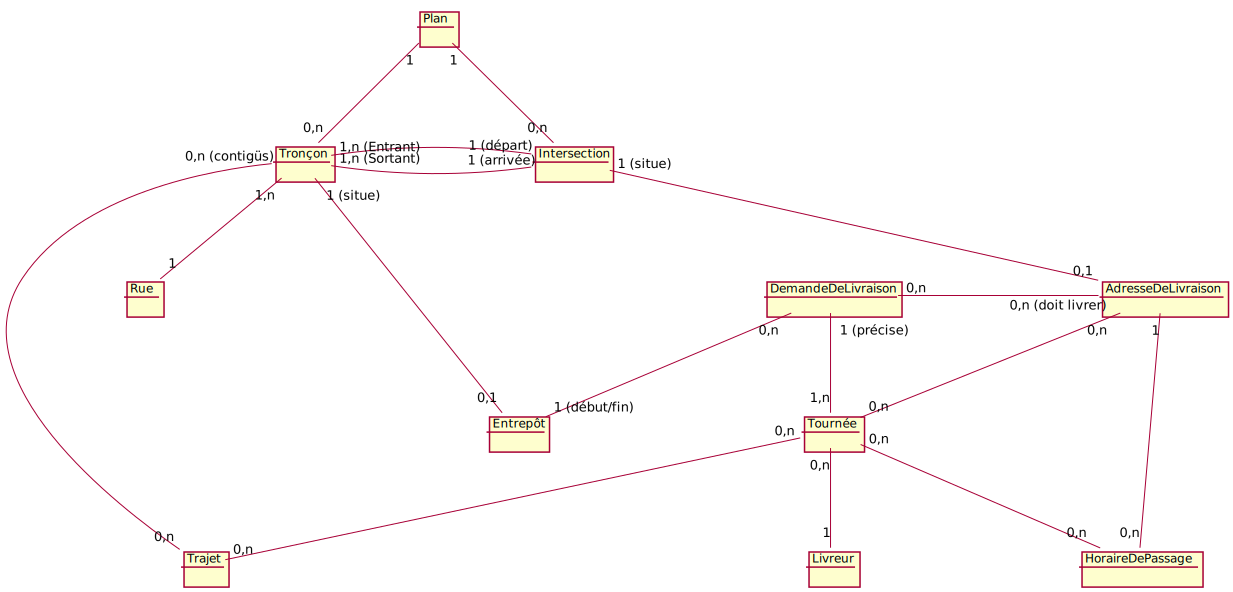
\includegraphics[width=\linewidth,height=.7\paperheight,keepaspectratio]{retrogenerated_uml/model.png}
      			\caption{Diagramme de classe du package model}
    		\end{center}
  	\end{figure}
\begin{figure}[h!]
    		\begin{center}
      			\includegraphics[width=\linewidth,height=.7\paperheight,keepaspectratio]{retrogenerated_uml/java.png}
      			\caption{Diagramme de classe du package java}
    		\end{center}
  	\end{figure}


\FloatBarrier
\input{docs/architecture.tex}


%mettre à jour les planning des différentes itérations
\FloatBarrier
%\section{Planning effectif de la première itération}
%  \begin{longtable}{|p{0.4\linewidth}|l|l|c|c|}
\caption{Répartition des charges} \label{tab:charges} \\

\hline
\multicolumn{1}{|c|}{\textbf{Nom de tâche}} & \multicolumn{1}{p{0.1\linewidth}|}{\textbf{Acteur principal}} & \multicolumn{1}{p{0.1\linewidth}|}{\textbf{Acteur aide}} & \multicolumn{1}{p{0.1\linewidth}|}{\textbf{Temps estimé (heures)}} & \multicolumn{1}{p{0.1\linewidth}|}{\textbf{Temps passé (heures)} } \\ \hline
\endfirsthead 

\multicolumn{5}{c}%
{{\bfseries \tablename\ \thetable{} -- suite du tableau précédant}} \\
\hline
\multicolumn{1}{|c|}{\textbf{Nom de tâche}} & \multicolumn{1}{p{0.1\linewidth}|}{\textbf{Acteur principal}} & \multicolumn{1}{p{0.1\linewidth}|}{\textbf{Acteur aide}} & \multicolumn{1}{p{0.1\linewidth}|}{\textbf{Temps estimé (heures)}} & \multicolumn{1}{p{0.1\linewidth}|}{\textbf{Temps passé (heures)}}                   \\ \hline
\endhead

\hline \multicolumn{5}{|r|}{{Suite sur la page suivante}} \\ \hline
\endfoot

\hline \hline
\endlastfoot


Glossaire                            & Ruben            & François    & 2                    & 2                   \\ \hline
Diagramme entité association         & François         & Ruben       & 2                    & 1                   \\ \hline
Modèle du domaine                    & François         & Ruben       & 3                    & 3                   \\ \hline
Diagramme de cas d'utilisations      & Nicolas          & Hugo        & 1                    & 1                   \\ \hline
Diagramme de cas d'utilisations      & Charles          & Sébastien   & 1                    & 1                   \\ \hline
Tenue des charges                    & Ruben            &             & 0,5                  & 0,5                 \\ \hline
Diagramme Etats-transitions          & Nicolas          & Hugo        & 0,5                  & 0,5                 \\ \hline
Diagramme Etats-transitions          & Charles          & Sébastien   & 0,5                  & 3                   \\ \hline
Diagramme de packages et de classes  & Nicolas          & Hugo        & 3                    & 1,5                 \\ \hline
Diagramme de packages et de classes  & Charles          & Sébastien   & 4                    & 5                   \\ \hline
Package Model                        & François         & Ruben       & 4                    & 2                   \\ \hline
Package Services                     & Ruben            & Nicolas     & 2                    & 2                   \\ \hline
Diagramme séquence TSP               & Ruben            &             & 1                    & 1                   \\ \hline
Diagramme séquence TSP global        & Charles          & Ruben       & 1                    & 2                   \\ \hline
Codage du Parser CityMap             & François         &             & 3                    & 3                   \\ \hline
Maquette de l'IHM                    & Sébastien        & Hugo        & 4                    & 4                   \\ \hline
Diagramme de classe (pck controller) & Charles          & Sébastien   & 4                    & 4                   \\ \hline
Diagramme de classe (pck controller) & Hugo             &             & 4                    & 4                   \\ \hline
Manage backlog                       & Ruben            &             & 1                    & 1                   \\ \hline
Note: backlog                        & Ruben            &             & 0,5                  & 1                   \\ \hline
Codage du Parser DeliveryRequest     & François         &             & 1,5                  & 3                   \\ \hline
Dijkstra                             & Sébastien        & François    & 5                    & 7                   \\ \hline
Implémentation TSP                   & Ruben            & Nicolas     & 2                    & 3                   \\ \hline
Implémentation computeDeliveryGraph  & Sébastien        &             & 1                    & 1                   \\ \hline
Test de Parser.getDeliveryRequest    & François         &             & 2                    & 3                   \\ \hline
Suppressions des wrappers du modele  & François         &             & 0,5                  & 0,5                 \\ \hline
Test de computeDeliveryGraph         & Sébastien        &             & 2                    & 2                   \\ \hline
Amélioration de shortestPath         & Sébastien        &             & 1                    & 1                   \\ \hline
Debug du TSP                         & Ruben            & François    & 2                    & 3                   \\ \hline
Mises en forme LaTeX                 & Nicolas          &             & 4                    & 5                   \\ \hline
Mise en place de la GUI              & Charles          &             & 3                    & 5                   \\ \hline
Composant "Application"              & Charles          & Hugo        & 5                    & 8                   \\ \hline
Composant "MapCanvas"                & Hugo             & Charles     & 4                    & 7                   \\ \hline
Composant "MapScreen"                & Charles          &             & 0.5                  & 0.5                 \\ \hline
Composant "PlanningDetails"          & Charles          &             & 2                    & 2.5                 \\ \hline
Outils (Intégration, Documentation)  & Charles          & Ruben       & 10                   & 15                  \\ \hline
\end{longtable}


\end{document}
